% !TeX spellcheck = en_US
%%%%%%%%%%%%%%%%%%%%%%%%%%%%%%%%%%%%%%%%%
%  My documentation report
%  Objetive: Explain what I did and how, so someone can continue with the investigation
%
% Important note:
% Chapter heading images should have a 2:1 width:height ratio,
% e.g. 920px width and 460px height.
%
%%%%%%%%%%%%%%%%%%%%%%%%%%%%%%%%%%%%%%%%%

%----------------------------------------------------------------------------------------
%	PACKAGES AND OTHER DOCUMENT CONFIGURATIONS
%----------------------------------------------------------------------------------------

\documentclass[12pt,fleqn,openany]{book} % Default font size and left-justified equations

\usepackage[top=3cm,bottom=3cm,left=3.2cm,right=3.2cm,headsep=10pt,a4paper]{geometry} % Page margins

\usepackage{xcolor} % Required for specifying colors by name
\definecolor{ocre}{RGB}{52,177,201} % Define the color used for highlighting throughout the book

% Font Settings
\usepackage{avant} % Use the Avantgarde font for headings
%\usepackage{times} % Use the Times font for headings
\usepackage{mathptmx} % Use the Adobe Times Roman as the default text font together with math symbols from the Sym­bol, Chancery and Com­puter Modern fonts
\usepackage{microtype} % Slightly tweak font spacing for aesthetics
\usepackage[utf8]{inputenc} % Required for including letters with accents
\usepackage[T1]{fontenc} % Use 8-bit encoding that has 256 glyphs
%\usepackage{indentfirst}
\usepackage{comment}
\usepackage{fmtcount} % equivalent to \usepackage[super]{nth}
\usepackage{siunitx}
\usepackage{subfig}
\usepackage{adjustbox}
\usepackage{wrapfig}
\usepackage{amsmath}
\usepackage{caption}
\usepackage{nomencl}
\makenomenclature

%----------------------------------------------------------------------------------------
%	VARIOUS REQUIRED PACKAGES
%----------------------------------------------------------------------------------------

\usepackage{titlesec} % Allows customization of titles

\usepackage{graphicx} % Required for including pictures
\graphicspath{{Pictures/}} % Specifies the directory where pictures are stored

\usepackage{lipsum} % Inserts dummy text

\usepackage{tikz} % Required for drawing custom shapes

\usepackage[english]{babel} % English language/hyphenation

\usepackage{enumitem} % Customize lists
\setlist{nolistsep} % Reduce spacing between bullet points and numbered lists

\usepackage{booktabs} % Required for nicer horizontal rules in tables

\usepackage{eso-pic} % Required for specifying an image background in the title page

%----------------------------------------------------------------------------------------
%	MAIN TABLE OF CONTENTS
%----------------------------------------------------------------------------------------

\usepackage{titletoc} % Required for manipulating the table of contents

\contentsmargin{0cm} % Removes the default margin
% Chapter text styling
\titlecontents{chapter}[1.25cm] % Indentation
{\addvspace{15pt}\large\sffamily\bfseries} % Spacing and font options for chapters
{\color{ocre!60}\contentslabel[\Large\thecontentslabel]{1.25cm}\color{ocre}} % Chapter number
{}  
{\color{ocre!60}\normalsize\sffamily\bfseries\;\titlerule*[.5pc]{.}\;\thecontentspage} % Page number
% Section text styling
\titlecontents{section}[1.25cm] % Indentation
{\addvspace{5pt}\sffamily\bfseries} % Spacing and font options for sections
{\contentslabel[\thecontentslabel]{1.25cm}} % Section number
{}
{\sffamily\hfill\color{black}\thecontentspage} % Page number
[]
% Subsection text styling
\titlecontents{subsection}[1.25cm] % Indentation
{\addvspace{1pt}\sffamily\small} % Spacing and font options for subsections
{\contentslabel[\thecontentslabel]{1.25cm}} % Subsection number
{}
{\sffamily\;\titlerule*[.5pc]{.}\;\thecontentspage} % Page number
[] 

%----------------------------------------------------------------------------------------
%	MINI TABLE OF CONTENTS IN CHAPTER HEADS
%----------------------------------------------------------------------------------------

% Section text styling
\titlecontents{lsection}[0em] % Indendating
{\footnotesize\sffamily} % Font settings
{}
{}
{}

% Subsection text styling
\titlecontents{lsubsection}[.5em] % Indentation
{\normalfont\footnotesize\sffamily} % Font settings
{}
{}
{}
 
%----------------------------------------------------------------------------------------
%	PAGE HEADERS
%----------------------------------------------------------------------------------------

\usepackage{fancyhdr} % Required for header and footer configuration

\pagestyle{fancy}
\renewcommand{\chaptermark}[1]{\markboth{\sffamily\normalsize\bfseries\ \thechapter.\ #1}{}} % Chapter text font settings
\renewcommand{\sectionmark}[1]{\markright{\sffamily\normalsize\thesection\hspace{5pt}#1}{}} % Section text font settings
\fancyhf{} \fancyhead[RE,RO]{\sffamily\normalsize\thepage} % Font setting for the page number in the header
%\fancyhead[LO]{\rightmark} % Print the nearest section name on the left side of odd pages
\fancyhead[LE,LO]{\leftmark} % Print the current chapter name on the right side of even pages
\renewcommand{\headrulewidth}{0.5pt} % Width of the rule under the header
\addtolength{\headheight}{2.5pt} % Increase the spacing around the header slightly
\renewcommand{\footrulewidth}{0pt} % Removes the rule in the footer
\fancypagestyle{plain}{\fancyhead{}\renewcommand{\headrulewidth}{0pt}} % Style for when a plain pagestyle is specified

% Removes the header from odd empty pages at the end of chapters
\makeatletter
\renewcommand{\cleardoublepage}{
\clearpage\ifodd\c@page\else
\hbox{}
\vspace*{\fill}
\thispagestyle{empty}
\newpage
\fi}



%----------------------------------------------------------------------------------------
%	THEOREM STYLES
%----------------------------------------------------------------------------------------

\usepackage{amsmath,amsfonts,amssymb,amsthm} % For math equations, theorems, symbols, etc

\newcommand{\intoo}[2]{\mathopen{]}#1\,;#2\mathclose{[}}
\newcommand{\ud}{\mathop{\mathrm{{}d}}\mathopen{}}
\newcommand{\intff}[2]{\mathopen{[}#1\,;#2\mathclose{]}}
\newtheorem{notation}{Notation}[chapter]

%%%%%%%%%%%%%%%%%%%%%%%%%%%%%%%%%%%%%%%%%%%%%%%%%%%%%%%%%%%%%%%%%%%%%%%%%%%
%%%%%%%%%%%%%%%%%%%% dedicated to boxed/framed environements %%%%%%%%%%%%%%
%%%%%%%%%%%%%%%%%%%%%%%%%%%%%%%%%%%%%%%%%%%%%%%%%%%%%%%%%%%%%%%%%%%%%%%%%%%
\newtheoremstyle{ocrenumbox}% % Theorem style name
{0pt}% Space above
{0pt}% Space below
{\normalfont}% % Body font
{}% Indent amount
{\small\bf\sffamily\color{ocre}}% % Theorem head font
{\;}% Punctuation after theorem head
{0.25em}% Space after theorem head
{\small\sffamily\color{ocre}\thmname{#1}\nobreakspace\thmnumber{\@ifnotempty{#1}{}\@upn{#2}}% Theorem text (e.g. Theorem 2.1)
\thmnote{\nobreakspace\the\thm@notefont\sffamily\bfseries\color{black}---\nobreakspace#3.}} % Optional theorem note
\renewcommand{\qedsymbol}{$\blacksquare$}% Optional qed square

\newtheoremstyle{blacknumex}% Theorem style name
{5pt}% Space above
{5pt}% Space below
{\normalfont}% Body font
{} % Indent amount
{\small\bf\sffamily}% Theorem head font
{\;}% Punctuation after theorem head
{0.25em}% Space after theorem head
{\small\sffamily{\tiny\ensuremath{\blacksquare}}\nobreakspace\thmname{#1}\nobreakspace\thmnumber{\@ifnotempty{#1}{}\@upn{#2}}% Theorem text (e.g. Theorem 2.1)
\thmnote{\nobreakspace\the\thm@notefont\sffamily\bfseries---\nobreakspace#3.}}% Optional theorem note

\newtheoremstyle{blacknumbox} % Theorem style name
{0pt}% Space above
{0pt}% Space below
{\normalfont}% Body font
{}% Indent amount
{\small\bf\sffamily}% Theorem head font
{\;}% Punctuation after theorem head
{0.25em}% Space after theorem head
{\small\sffamily\thmname{#1}\nobreakspace\thmnumber{\@ifnotempty{#1}{}\@upn{#2}}% Theorem text (e.g. Theorem 2.1)
\thmnote{\nobreakspace\the\thm@notefont\sffamily\bfseries---\nobreakspace#3.}}% Optional theorem note

%%%%%%%%%%%%%%%%%%%%%%%%%%%%%%%%%%%%%%%%%%%%%%%%%%%%%%%%%%%%%%%%%%%%%%%%%%%
%%%%%%%%%%%%% dedicated to non-boxed/non-framed environements %%%%%%%%%%%%%
%%%%%%%%%%%%%%%%%%%%%%%%%%%%%%%%%%%%%%%%%%%%%%%%%%%%%%%%%%%%%%%%%%%%%%%%%%%
\newtheoremstyle{ocrenum}% % Theorem style name
{5pt}% Space above
{5pt}% Space below
{\normalfont}% % Body font
{}% Indent amount
{\small\bf\sffamily\color{ocre}}% % Theorem head font
{\;}% Punctuation after theorem head
{0.25em}% Space after theorem head
{\small\sffamily\color{ocre}\thmname{#1}\nobreakspace\thmnumber{\@ifnotempty{#1}{}\@upn{#2}}% Theorem text (e.g. Theorem 2.1)
\thmnote{\nobreakspace\the\thm@notefont\sffamily\bfseries\color{black}---\nobreakspace#3.}} % Optional theorem note
\renewcommand{\qedsymbol}{$\blacksquare$}% Optional qed square
\makeatother

% Defines the theorem text style for each type of theorem to one of the three styles above
\newcounter{dummy} 
\numberwithin{dummy}{section}
\theoremstyle{ocrenumbox}
\newtheorem{theoremeT}[dummy]{Theorem}
\newtheorem{problem}{Problem}[chapter]
\newtheorem{exerciseT}{Exercise}[chapter]
\theoremstyle{blacknumex}
\newtheorem{exampleT}{Example}[chapter]
\theoremstyle{blacknumbox}
\newtheorem{vocabulary}{Vocabulary}[chapter]
\newtheorem{definitionT}{Definition}[section]
\newtheorem{corollaryT}[dummy]{Corollary}
\theoremstyle{ocrenum}
\newtheorem{proposition}[dummy]{Proposition}

%----------------------------------------------------------------------------------------
%	DEFINITION OF COLORED BOXES
%----------------------------------------------------------------------------------------

\RequirePackage[framemethod=default]{mdframed} % Required for creating the theorem, definition, exercise and corollary boxes

% Theorem box
\newmdenv[skipabove=7pt,
skipbelow=7pt,
backgroundcolor=black!5,
linecolor=ocre,
innerleftmargin=5pt,
innerrightmargin=5pt,
innertopmargin=5pt,
leftmargin=0cm,
rightmargin=0cm,
innerbottommargin=5pt]{tBox}

% Exercise box	  
\newmdenv[skipabove=7pt,
skipbelow=7pt,
rightline=false,
leftline=true,
topline=false,
bottomline=false,
backgroundcolor=ocre!10,
linecolor=ocre,
innerleftmargin=5pt,
innerrightmargin=5pt,
innertopmargin=5pt,
innerbottommargin=5pt,
leftmargin=0cm,
rightmargin=0cm,
linewidth=4pt]{eBox}	

% Definition box
\newmdenv[skipabove=7pt,
skipbelow=7pt,
rightline=false,
leftline=true,
topline=false,
bottomline=false,
linecolor=ocre,
innerleftmargin=5pt,
innerrightmargin=5pt,
innertopmargin=0pt,
leftmargin=0cm,
rightmargin=0cm,
linewidth=4pt,
innerbottommargin=0pt]{dBox}	

% Corollary box
\newmdenv[skipabove=7pt,
skipbelow=7pt,
rightline=false,
leftline=true,
topline=false,
bottomline=false,
linecolor=gray,
backgroundcolor=black!5,
innerleftmargin=5pt,
innerrightmargin=5pt,
innertopmargin=5pt,
leftmargin=0cm,
rightmargin=0cm,
linewidth=4pt,
innerbottommargin=5pt]{cBox}

% Creates an environment for each type of theorem and assigns it a theorem text style from the "Theorem Styles" section above and a colored box from above
\newenvironment{theorem}{\begin{tBox}\begin{theoremeT}}{\end{theoremeT}\end{tBox}}
\newenvironment{exercise}{\begin{eBox}\begin{exerciseT}}{\hfill{\color{ocre}\tiny\ensuremath{\blacksquare}}\end{exerciseT}\end{eBox}}				  
\newenvironment{definition}{\begin{dBox}\begin{definitionT}}{\end{definitionT}\end{dBox}}	
\newenvironment{example}{\begin{exampleT}}{\hfill{\tiny\ensuremath{\blacksquare}}\end{exampleT}}		
\newenvironment{corollary}{\begin{cBox}\begin{corollaryT}}{\end{corollaryT}\end{cBox}}	

%----------------------------------------------------------------------------------------
%	REMARK ENVIRONMENT
%----------------------------------------------------------------------------------------

\newenvironment{remark}{\par\vspace{10pt}\small % Vertical white space above the remark and smaller font size
\begin{list}{}{
\leftmargin=35pt % Indentation on the left
\rightmargin=25pt}\item\ignorespaces % Indentation on the right
\makebox[-2.5pt]{\begin{tikzpicture}[overlay]
\node[draw=ocre!60,line width=1pt,circle,fill=ocre!25,font=\sffamily\bfseries,inner sep=2pt,outer sep=0pt] at (-15pt,0pt){\textcolor{ocre}{R}};\end{tikzpicture}} % Orange R in a circle
\advance\baselineskip -1pt}{\end{list}\vskip5pt} % Tighter line spacing and white space after remark

%----------------------------------------------------------------------------------------
%	SECTION NUMBERING IN THE MARGIN
%----------------------------------------------------------------------------------------

\makeatletter
\renewcommand{\@seccntformat}[1]{\llap{\textcolor{ocre}{\csname the#1\endcsname}\hspace{1em}}}                    
\renewcommand{\section}{\@startsection{section}{1}{\z@}
{-4ex \@plus -1ex \@minus -.4ex}
{1ex \@plus.2ex }
{\normalfont\large\sffamily\bfseries}}
\renewcommand{\subsection}{\@startsection {subsection}{2}{\z@}
{-3ex \@plus -0.1ex \@minus -.4ex}
{0.5ex \@plus.2ex }
{\normalfont\sffamily\bfseries}}
\renewcommand{\subsubsection}{\@startsection {subsubsection}{3}{\z@}
{-2ex \@plus -0.1ex \@minus -.2ex}
{.2ex \@plus.2ex }
{\normalfont\small\sffamily\bfseries}}                        
\renewcommand\paragraph{\@startsection{paragraph}{4}{\z@}
{-2ex \@plus-.2ex \@minus .2ex}
{.1ex}
{\normalfont\small\sffamily\bfseries}}

%----------------------------------------------------------------------------------------
%	HYPERLINKS IN THE DOCUMENTS
%----------------------------------------------------------------------------------------

% For an unclear reason, the package should be loaded now and not later
\usepackage{hyperref}
\hypersetup{hidelinks,backref=true,pagebackref=true,hyperindex=true,colorlinks=false,breaklinks=true,urlcolor= ocre,bookmarks=true,bookmarksopen=false,pdftitle={Title},pdfauthor={Author}}

%----------------------------------------------------------------------------------------
%	CHAPTER HEADINGS
%----------------------------------------------------------------------------------------

% The set-up below should be (sadly) manually adapted to the overall margin page septup controlled by the geometry package loaded in the main.tex document. It is possible to implement below the dimensions used in the goemetry package (top,bottom,left,right)... TO BE DONE

\newcommand{\thechapterimage}{}
\newcommand{\chapterimage}[1]{\renewcommand{\thechapterimage}{#1}}

% Numbered chapters with mini tableofcontents
\def\thechapter{\arabic{chapter}}
\def\@makechapterhead#1{
\thispagestyle{empty}
{\centering \normalfont\sffamily
\ifnum \c@secnumdepth >\m@ne
\if@mainmatter
\startcontents
\begin{tikzpicture}[remember picture,overlay]
\node at (current page.north west)
{\begin{tikzpicture}[remember picture,overlay]
%\node[anchor=north west,inner sep=0pt] at (0,0) {\includegraphics[width=\paperwidth]{\thechapterimage}};
%%%%%%%%%%%%%%%%%%%%%%%%%%%%%%%%%%%%%%%%%%%%%%%%%%%%%%%%%%%%%%%%%%%%%%%%%%%%%%%%%%%%%
% Commenting the 3 lines below removes the small contents box in the chapter heading
%\fill[color=ocre!10!white,opacity=.6] (1cm,0) rectangle (8cm,-7cm);
%\node[anchor=north west] at (1.1cm,.35cm) {\parbox[t][8cm][t]{6.5cm}{\huge\bfseries\flushleft \printcontents{l}{1}{\setcounter{tocdepth}{2}}}};
\draw[anchor=west] (5cm,-3cm) node [rounded corners=20pt,fill=ocre!10!white,text opacity=1,draw=ocre,draw opacity=1,line width=1.5pt,fill opacity=.6,inner sep=12pt]{\huge\sffamily\bfseries\textcolor{black}{\thechapter. #1\strut\makebox[22cm]{}}};
%%%%%%%%%%%%%%%%%%%%%%%%%%%%%%%%%%%%%%%%%%%%%%%%%%%%%%%%%%%%%%%%%%%%%%%%%%%%%%%%%%%%%
\end{tikzpicture}};
\end{tikzpicture}}
\par\vspace*{40\p@}
\fi
\fi}

% Unnumbered chapters without mini tableofcontents (could be added though) 
\def\@makeschapterhead#1{
\thispagestyle{empty}
{\centering \normalfont\sffamily
\ifnum \c@secnumdepth >\m@ne
\if@mainmatter
\begin{tikzpicture}[remember picture,overlay]
\node at (current page.north west)
{\begin{tikzpicture}[remember picture,overlay]
%\node[anchor=north west,inner sep=0pt] at (0,0) {\includegraphics[width=\paperwidth]{\thechapterimage}};
\draw[anchor=west] (5cm,-3cm) node [rounded corners=20pt,fill=ocre!10!white,fill opacity=.6,inner sep=12pt,text opacity=1,draw=ocre,draw opacity=1,line width=1.5pt]{\huge\sffamily\bfseries\textcolor{black}{#1\strut\makebox[22cm]{}}};
\end{tikzpicture}};
\end{tikzpicture}}
\par\vspace*{40\p@}
\fi
\fi
}
\makeatother % Insert the commands.tex file which contains the majority of the structure behind the template
\newcommand{\e}[1]{\cdot 10^{#1}}

\begin{document}
	
%----------------------------------------------------------------------------------------
%	TITLE PAGE
%----------------------------------------------------------------------------------------
\begin{titlepage}
\begin{center}
\sffamily
\textsc{\Huge\bfseries Politecnico di Milano}\\[1.5cm] % Name of your university/college
\LARGE{\bfseries Thrust Imbalance Analysis\\ Ariane 5 ECA}\\[0.5cm]  % Title
\textsc{\LARGE  Launch Systems}\\ % Major heading such as course name
%\large {Dipartimento di Scienze e Tecnologie Aerospaziali - DAER}\\[1.5cm] % Minor heading such as course title
\large {Aerospace Science and Technology Department- DAER}\\[1.5cm] % Minor heading such as course title
%----------------------------------------------------------------------------------------
%	AUTHOR SECTION
%----------------------------------------------------------------------------------------
\begin{flushright}
	\large
	\emph{Authors:}\\
	[0.5cm]
	Nicolò \textsc{\bfseries{Bramani}} 883811\\ % Your name
	Alessandro Maria \textsc{\bfseries{Masserini}}  883251\\ % Your name
	Alessio \textsc{\bfseries{Negri}}	874935\\ % Your name
	Pierfrancesco \textsc{\bfseries{Pansini}} 885031\\ % Your name
	Marcello \textsc{\bfseries{Scalera}} 874378\\ % Your name
	Alberto \textsc{\bfseries{Sedini}} 883472\\ % Your name
	\textsc{\bfseries{Group: 3}}\\
	[1cm]
	\emph{Supervisor:} \\
	[0.5cm]
	Prof. Filippo \textsc{\bfseries{Maggi}}\\ % Supervisor's Name
	[1cm]
\end{flushright}
%----------------------------------------------------------------------------------------
%	LOGO SECTION
%----------------------------------------------------------------------------------------

\includegraphics[scale=0.6]{Logo.png}\\[1.5cm] % Include a department/university logo - this will require the graphicx package
%----------------------------------------------------------------------------------------
%	DATE SECTION
%----------------------------------------------------------------------------------------
{\large A.Y. 2017/2018 - December 2017}\\[3cm] % Date, change the \today to a set date if you want to be precise
%----------------------------------------------------------------------------------------
\vfill % Fill the rest of the page with whitespace
\end{center}
\end{titlepage}
%----------------------------------------------------------------------------------------
%	TABLE OF CONTENTS
%----------------------------------------------------------------------------------------
\pagestyle{empty} % No headers
\chapter*{Abstract}
This report contains the results of the analysis of the thrust imbalance between the twin external solid rocket motors (SRMs) used on the \textbf{Ariane 5 ECA}. All the real characteristics of the rocket (geometry, masses, deflection angles limits, …) have been taken. A first analysis of the aerodynamic, propulsion and mass distribution was performed to develop the thrust imbalance study. The study is focused on the thrust vector control (TVC) system, consisting on the movable nozzles of the two boosters and the central liquid rocket engine. The two SRM thrusts are modelled with two different rectangular distributions and then the resulting imbalance is evaluated to give more generality to its formation. The report will cover many important aspects regarding the launcher starting from a managerial study of the project through a \textit{House of Quality} analysis and a project triangular scheme. The results obtained are then compared to the limiting angles to see if they are overcome. Two critical conditions are considered: maximum SRM thrust and maximum dynamic pressure. At the end, the TVC systems are able to counteract a normal force for small angles of attack, in which the rocket typically works. \tableofcontents % Print the table of contents itself

\pagestyle{fancy} % Print headers again

%\begin{comment}
%----------------------------------------------------------------------------------------
%	LIST OF TABLES
%----------------------------------------------------------------------------------------

\pagestyle{empty} % No headers

\listoftables

\pagestyle{fancy} % Print headers again

%----------------------------------------------------------------------------------------
%	LIST OF FIGURES
%----------------------------------------------------------------------------------------

\pagestyle{empty} % No headers

\listoffigures

\pagestyle{fancy} % Print headers again

%\end{comment}

% \chapter*{List of Symbols}
% \begin{table}[h]
% 	\centering
% 	\begin{tabular}{ l l l }		% Alphabetical order
% 		\toprule
% 		\textbf{Symbol} & \textbf{Description} & \textbf{UOM}  \\
% 		\midrule
		
		\nomenclature{$C_d         $ 		}{Zero-Lift Drag Coefficient                                                            }%&\si{}                 	\\
        \nomenclature{$M		     $      }{Mach Number                                                                 }%&\si{}                 	\\
        \nomenclature{$C_N 		 $          }{Normal Aerodynamic Force Coefficient                                          }%&\si{}                 	\\
        \nomenclature{$C_{N/\alpha}$	    }{Derivative of Normal Aerodynamic Force Coefficient with respect to $\alpha$ }%&\si{}                 	\\
        \nomenclature{$a 		     $      }{Semi-major axis of the lifting body                                         }%&\si{\meter}           	\\
        \nomenclature{$b 		     $      }{Semi-minor axis of the lifting body                                         }%&\si{\meter}           	\\
        \nomenclature{$\phi 		 $      }{Bank angle                                                                  }%&\si{\radian}          	\\
        \nomenclature{$\alpha		 $      }{Angle of Attack                                                             }%&\si{\radian}          	\\
        \nomenclature{$l 		     $      }{Generic Length                                                              }%&\si{\meter}           	\\
        \nomenclature{$d 		     $      }{Generic diameter                                                            }%&\si{\meter}           	\\
        \nomenclature{$d_m 		 $          }{Minimum Diameter                                                            }%&\si{\meter}           	\\
        \nomenclature{$S 		     $      }{Reference surface                                                           }%&\si{\meter\squared}   	\\
        \nomenclature{$S_b 		 $          }{Base surface                                                                }%&\si{\meter\squared}   	\\
        \nomenclature{$h 		     $      }{Generic height of the nose                                                  }%&\si{\meter}           	\\
        \nomenclature{$l_B 		 $          }{Body length                                                                 }%&\si{\meter}           	\\
        \nomenclature{$l_N 		 $          }{Nose length                                                                 }%&\si{\meter}           	\\
        \nomenclature{$l_{EAP} 		$       }{Booster length                                                              }%&\si{\meter}           	\\
        \nomenclature{$h_f 		 $          }{Flare length                                                                }%&\si{\meter}           	\\
        \nomenclature{$d_{EAP}  		$   }{Booster diameter                                                            }%&\si{\meter}           	\\
        \nomenclature{$d_{EPC}  		$   }{Main core stage diameter                                                    }%&\si{\meter}           	\\
        \nomenclature{$x_{cp}^{EAP}$ 	    }{Centre of pressure position of the booster from the nose                    }%&\si{\meter}            \\
        \nomenclature{$x_{cp}^{EPC}$ 	    }{Centre of pressure position of the main core stage from the nose            }%&\si{\meter}            \\
        \nomenclature{$x_{cp} 		$       }{Centre of pressure of the launcher from the nose                            }%&\si{\meter}       		\\
        \nomenclature{$A_{EAP} 		$       }{Booster Surface                                                             }%&\si{\meter\squared}   	\\
        \nomenclature{$A_f 		 $          }{Flare Surface                                                               }%&\si{\meter\squared}   	\\
        \nomenclature{$M_{prop}  	$       }{Propellant mass                                                             }%&\si{\kilogram}        	\\
        \nomenclature{$\dot{m}_{prop}$ 	    }{propellant mass flow rate                                                   }%&\si{\kilogram}     	\\
        \nomenclature{$\delta_{EPC} 	$   }{Deflection angle of the main core stage nozzle                              }%&\si{\radian}          	\\
        \nomenclature{$\delta_{EAP1} $	    }{Deflection angle of the left booster nozzle                                 }%&\si{\radian}       	\\
        \nomenclature{$\delta_{EAP2} $	    }{Deflection angle of the right booster nozzle                                }%&\si{\radian}       	\\
        \nomenclature{$T_1 		   $        }{Thrust of the left booster                                                  }%&\si{\newton}          	\\
        \nomenclature{$T_2 		   $        }{Thrust of the right booster                                                 }%&\si{\newton}          	\\
        \nomenclature{$\Delta T_1 	  $     }{Percentage random variation of the left booster thrust                      }%&\si{}             		\\
        \nomenclature{$\Delta T_2	   $    }{Percentage random variation of the right booster thrust                     }%&\si{}                 	\\
        \nomenclature{$\Delta T 		  $ }{Total percentage random variation of the thrust                             }%&\si{}                 	\\
        \nomenclature{$T_{EAP} 		  $     }{Thrust of the boosters                                                      }%&\si{\newton}          	\\
        \nomenclature{$CG 		   $        }{Centre of gravity position from the base                                    }%&\si{\meter}       		\\
        \nomenclature{$CP-CG 	   $        }{Distance between the centre of pressure and the centre of gravity                                   }%&\si{\meter}       		\\
        \nomenclature{$N 		       $    }{Normal Aerodynamic Force                                                    }%&\si{\newton}          	\\
        \nomenclature{$q 		       $    }{Dynamic Pressure                                                            }%&\si{\newton/\meter\squared}\\
        \nomenclature{$\bar{y} 	   $        }{Distance from symmetry axis to compute the torque                           }%&\si{\meter}           	\\
        \nomenclature{$T_{ideal} 	 	 $  }{Ideal Thrust                                                                }%&\si{\newton}          	\\
        \nomenclature{$T_{EPC} 		  $     }{Main Core Thrust                                                            }%&\si{\newton}          	\\
        \nomenclature{$A_{ref} 		  $     }{Reference Area                                                              }%&\si{\meter\squared}   	\\
        \nomenclature{$m_{fairing}	  $     }{Fairing mass                                                                }%&\si{\kilogram}    		\\
        \nomenclature{$m_{ESC-A}	   $    }{Second stage mass                                                           }%&\si{\kilogram}        	\\
        \nomenclature{$m_s^{EPC}	   $    }{Main stage structural mass                                                  }%&\si{\kilogram}        	\\
        \nomenclature{$m_s^{EAP}	   $    }{Booster structural mass                                                     }%&\si{\kilogram}        	\\
        \nomenclature{$R_u	   $    }{Universal gas constant                                                     }%&\si{\kilogram}        	\\

% 		\bottomrule
% 	\end{tabular}
% 	\caption{List of Symbols}
% 	\label{tab:sym}
% \end{table}


%----------------------------------------------------------------------------------------
%	CHAPTERS
%----------------------------------------------------------------------------------------
                                  \printnomenclature
\chapter{Introduction}
Thrust imbalance is an important issue in case of external solid rocket motors. The rocket launcher under study is the \textbf{Ariane 5 ECA}, which has been chosen as baseline, and as competitors \textit{Falcon Heavy} and \textit{Delta IV Heavy}. Its origin has been studied for different rockets. A first study was performed on the Space Shuttle solid rocket motors \cite{bib:1},\cite{bib:2}. These studies performed Monte Carlo simulations to see the resulting thrust imbalance in two cases: ignition and transients. The nature of the imbalance is related to the internal behaviour of the motor. They introduced random variations for the main variables defining the propulsion parameters from which the thrust has been evaluated for the couple of motors, and then they have simulated the thrust imbalance. Also, recent works has been done, as the one on the Space Launch System by NASA \cite{bib:3}. The main effect due to thrust imbalance considered in this study can be explained as a disturbance moment generated by an off-design performance of the boosters. The resulting couple of the solid boosters’ thrusts tends to make the rocket turn. In design conditions, the moments generated by the boosters are perfectly balanced between themselves; in real applications, some disturbances may cause the generation of the imbalance effect even if boosters are working near to optimal performance condition. TVC is used to compensate the rotation and to follow the desired attitude during the launch. A normal aerodynamic force \textit{N} has been introduced to be counteracted by the TVC systems, in addition to the imbalance. Different levels of \textit{N} are analysed, changing the angle of attack. The thrust losses are modelled as random variations of thrust levels that can be expressed statistically as a rectangular distribution around the average nominal value. The study is focused on the boosting phase explaining briefly the ideal case and providing an insight of a hypothetic thrust imbalance scenario due to possible engine issues to both the solid boosters, leading to thrust variations in a range between $\pm\SI{5}{\%}$. For this analysis have been used different software: Matlab\textsuperscript\textregistered, for the simulations and parameters computations, SolidWorks\textsuperscript\textregistered, for the model creation and the mass distribution, CEA by NASA, for propulsive computations and the \textit{WebPlotDigitalizer} tool to extrapolate data from drawn charts.\chapter{Requirements and Specifications}
\section{Requirements}
The customer requirements [relative weight] are: 
\begin{itemize}
 \item \textit{Similar-to-target altitude and velocity at boosters’ detachment }[30.3\%]: due to an imbalance in the thrust the preliminary target can be unreachable and an acceptable similar one should be reached. 
\item \textit{Full control of trajectory} [24.2\%]: during the whole flight, the rocket trajectory must be fully controllable. 
\item \textit{High precision attitude control} [21.2\%]: to manage the thrust imbalance an effective attitude control system is required. 
\item \textit{Lightweight system} [6.1\%]: a lightweight system is preferable due to many advantages. 
\item \textit{Cheap system} [6.1\%]. 
\item \textit{Robustness to atmospheric disturbances} [12.1\%]:  a minor effect of atmospheric disturbances (e.g. transversal winds) should help in focusing on the management of thrust imbalance. 
 \end{itemize}
\section{Specifications}
\subsection{Project management triangle}
As managerial approach, the best decision results in focusing on performances and time, with a minimum weak limitation on cost. In terms of performances it’s needed to fulfil the customer requirements; in addition, in order to achieve those requirements a fast approach has been selected. The scheme is shown in figure \hypertarget{fig:triang}{\ref{fig:triang}}. 
\begin{figure}[h]
 \centering
 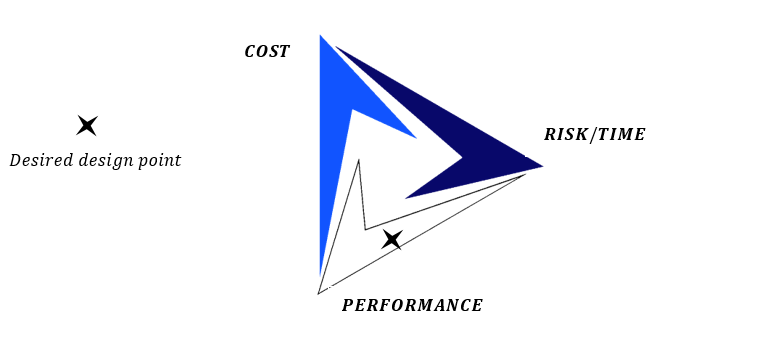
\includegraphics[width=0.85\textwidth]{triang}
 \caption{\emph{Project management triangle}}
 \label{fig:triang}
\end{figure}
\newpage
\subsection{Functional requirements}
The functional requirements [relative weight] are: 
\begin{itemize}
 \item \textit{TVC angle excursion} [13.0\%]: a higher angle is preferable to obtain a larger controllability window for rocket attitude dynamics. 
\item \textit{Aerodynamic drag} [4.0\%]:  a low aerodynamic effect is important to reduce stresses and losses. 
\item \textit{Sustainer thrust fraction} [4.6\%]:  a higher fraction would guarantee a minor sensibility to boosting phase imbalance, however losses due to parallel configuration are increased. 
\item \textit{Boosters thrust fraction} [10.1\%]:  a higher fraction would cause a major sensibility to boosting phase imbalance, but it would grant a smaller system due to a lower propellant volume. 
\item \textit{Centre of mass excursion} [5.1\%]. 
\item \textit{Misalignment of thrust with respect to centre of mass} [9.8\%]: the boosting phase unbalance generates an arm for the vertical component of thrust, that causes an undesired moment. 
\item \textit{Velocity at boosters’ detachment} [7.8\%]. 
\item \textit{Altitude at boosters’ detachment} [9.1\%]. 
\item \textit{Sensors responding time} [13.7\%]. 
\item \textit{Attitude angular position sensitivity} [10.1\%]: parameter that defines how much sensors’ sensitivity to angular position affects the precision in attitude reconstruction. 
\item \textit{Attitude angular velocity sensitivity} [10.1\%]: parameter that defines how much sensors’ sensitivity to angular velocity affects the precision in attitude reconstruction. 
\item \textit{GPS/Radar visibility} [2.6\%]: important parameter to keep track of the rocket during its flight trajectory.  
\end{itemize}

\subsection{Competitive analysis}
Two main competitors to \textbf{Ariane 5 ECA} are considered:
\begin{enumerate}
 \item \textbf{SpaceX} – \textit{Falcon Heavy}
 \item \textbf{Nasa} – \textit{Delta IV Heavy}
\end{enumerate}
As shown in figure \hypertarget{fig:hoq}{\ref{fig:hoq}}, the strongest competitor is the \textit{Falcon Heavy} which assures higher performances in most of the customer requirements. However, \textit{Falcon Heavy} has never flown in a real mission and because of this its data are just theoretical. The \textit{Delta IV Heavy} has accomplished many missions, but it has lower performances in all the meaningful mission parameters exception made for the lightweight system parameter.
\newpage
\subsection{House of Quality analysis}
\begin{figure}[h]
 \centering
 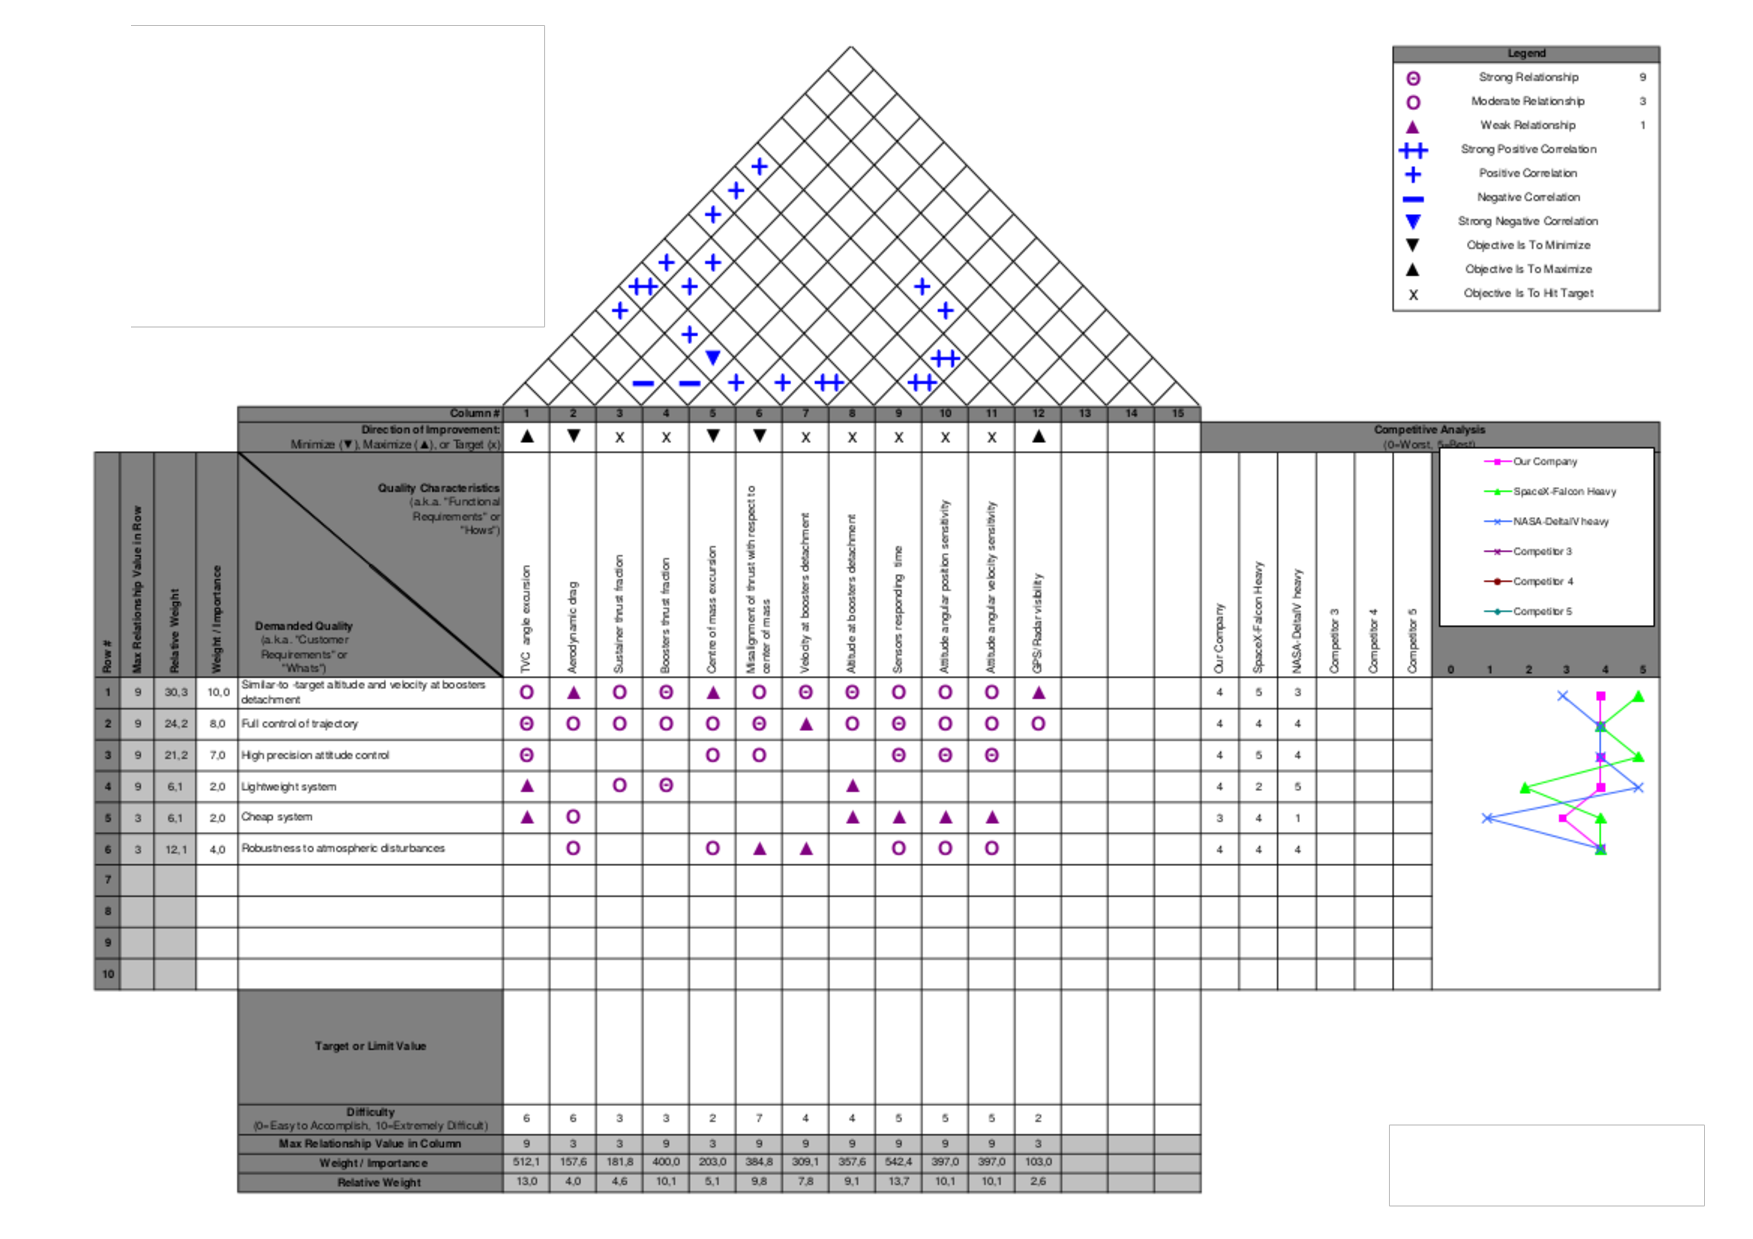
\includegraphics[width=1.2\textwidth,angle=270]{hoq}
 \caption{\emph{HOQ analysis}}
 \label{fig:hoq}
\end{figure}

\noindent The \textit{House of Quality} results are shown in figure \hypertarget{fig:hoq}{\ref{fig:hoq}}. The most important functional requirements according to the \textit{House of Quality} are \textbf{Sensor Responding Time} (13.7\% with respect to the weight of all the other ones) and \textbf{TVC angle excursion} (with a relative weight of 13.0\%). In addition, precision in the attitude determination is an important parameter and it is defined by two tied requirements in third place (10.1\% for \textbf{Attitude Angular Velocity Sensitivity} and \textbf{Attitude Angular Position Sensitivity}). Moreover, \textbf{Boosters thrust fraction} is tied at 10.1\% and it affects the attitude control and determination because the lower is their thrust fraction, the lower will be also the imbalance generated by them. All the other functional requirements have lower relative weights that make them of low importance to this study. Suitable time of response and high precision of the sensors are essential in order to reconstruct the attitude of the system, while a suitable TVC control system is strictly needed to correct the attitude and to follow the desired configuration. The combination of these two requirements leads to an effective active attitude control of the launcher able to counteract imbalance effects. In our analysis, a proper attitude reconstruction by sensors data is assumed as given and the whole work is focused on the use of TVC system, by verifying that it's able to work in critical conditions.  
\subsection{Baseline}
\textbf{Ariane 5 ECA} in the nominal condition is the baseline for this study. The nominal system is composed by a parallel first stage with a liquid cryogenic couple $LH_2/LOX$ main engine and two solid rocket boosters that provide almost 90\% of the total thrust at lift-off. There is also a cryogenic upper stage, but it is of no interest for this project. All the data,taken from \cite{bib:4}, \cite{bib:5}, \cite{bib:6} are listed in table **. All the additional parameters needed for this study (aerodynamic, propulsion, mass distribution, …) will be evaluated next.
\begin{table}[h]
	\centering
	\begin{tabular}{ l c c}
		\toprule
		Symbol									&Value 				&UOM	\\
		\midrule                                                                                                             
		$l_B  		$							&$50.5  $          &\si{\meter}        \\  
		$l_N  		$							&$7     $          &\si{\meter}        \\  
		$l_F  		$							&$17    $          &\si{\meter}        \\  
		$l_{ESCA}  	$							&$4.711 $          &\si{\meter}        \\
		$l_{EPC}  	$								&$23.8  $      &\si{\meter}        \\    
		$l_{EAP}  	$								&$30    $      &\si{\meter}        \\    
		$l_{N_EAP}  	$							&$4.375 $      &\si{\meter}        \\  
		$x_f  		$							&$28.98 $          &\si{\meter}        \\  
		$d_c  		$							&$1     $          &\si{\meter}        \\  
		$d_{ESCA}  	$							&$5.4   $          &\si{\meter}        \\
		$d_{EPC } 	$								&$5.4	$      &\si{\meter}        \\    
		$d_{EAP } 	$								&$3.05  $      &\si{\meter}        \\    
		$d_f  		$							&$3.10  $          &\si{\meter}        \\  
		$h_f  		$							&$1.02  $          &\si{\meter}        \\  
		$d_m  		$							&$3.075 $          &\si{\meter}        \\
		$a$										&$5.75$            &\si{\meter}        \\
		$b$                                     &$2.70$            &\si{\meter}        \\
		$d_{e_{EAP}}$ 								&$3.10$     	   &\si{\meter}        \\
		$A_{ref}$								&$37.51$		   &\si{\meter\squared}\\
		$M_F  		$							&$12675 $          &\si{\kilogram}     \\
		$M_{ESCA } 	$							&$19440 $          &\si{\kilogram}     \\
		$M_{EPC  }	$								&$171500$      &\si{\kilogram}     \\
		$M_{EAP  }	$								&$275000$      &\si{\kilogram}     \\
		\bottomrule
	\end{tabular} 
	\caption{\emph{Geometry and mass data}}
	\label{tab:gmdata}
\end{table}

\begin{table}[h]
	\centering
	\begin{tabular}{ l c c}
		\toprule
		Symbol									&Value 				&UOM	\\
		\midrule                                                                                                             
		$I_{sp_{SL}}  	$						&$262    $			&\si{\second}                       \\
		$I_{sp_{vac}} 	$						&$274.5  $			&\si{\second}                       \\
		$g_0			$							&$9.81   $		&	\si{\meter\over\second\squared}\\
		$m_{prop}   		$						&$173300 $		&	\si{\kilogram}					\\
		$e_{ratio}		$							&$61.5   $		&	\si{}                           \\
		$\gamma			$					    &$1.2873 $			&\si{}                               \\
		$P_{cc}			$						    &$116e5  $		&	\si{\pascal}                    \\
		$T_{cc}			$						    &$3539.57$		&	\si{\kelvin}                    \\
		$m_{mol}    		$						&$13.534 $		&	\si{\kilogram\over\mole}            \\
		$m_p      		$						&$175000 $			&\si{\kilogram}                      \\
		$t_{burn}   		$						&$540    $		&	\si{\second}                    \\
		$o/f$									&$6$  \\
		\bottomrule
	\end{tabular} 
	\caption{\emph{Propulsion data}}
	\label{tab:prdata}
\end{table}
% \begin{table}[h]
% 	\centering
% 	\begin{tabular}{ lcccccl }
% \toprule
% Stage       	&Weight at lift-off  	&Thrust SL      &Thrust vac   &$I_{sp_{SL}}$    &$I_{sp-vac}$        &Chemical composition\\
% 		&[tons]		&[kN]	&[kN]    &[s]  &[s]                    \\
% \midrule                                                                                                             
% EPC		&$184.4$             &$916.92$    &$1299.24$ &$291.24$ &$412.68$ &LH2/LOX             \\                                                 
% EAP	        &$240.0$             &$6487.67$   &$5997.62$ &$262.0$  &$274.5$  &HTPB                \\
% \bottomrule
% \end{tabular} 
% \caption{Baseline}
% \label{tab:baseline}
% \end{table}


\chapter{Aerodynamics}
In this chapter it will be analysed the \textbf{Ariane 5 ECA} rocket aerodynamics. Aerodynamics is a very complex aspect to model during a design phase, and the behaviour of the flow around a rocket is very complicated and difficult to foresee. In this case the configuration of a parallel rocket complicates more the study. The model of the rocket has been created with SolidWorks\textsuperscript\textregistered using the real dimensions and masses [figure \hypertarget{fig:A5s}{\ref{fig:A5s}}]. The main aspect analysed are the zero-lift drag coefficient, the normal force coefficient (useful for the thrust vector control) and the position of the centre of pressure (useful for the thrust vector control). 
\begin{figure}[h]
 \centering
 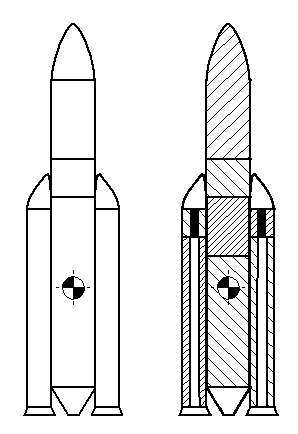
\includegraphics[width=0.5\textwidth]{A5scheme}
 \caption{\emph{Ariane 5 ECA scheme: outside view (left) and inside view (right)}}
 \label{fig:A5s}
\end{figure}
\section{Drag coefficient}
First, the zero-lift drag coefficient of the rocket is evaluated. Using the \textit{WebPlotDigitalizer} tool, from our baseline is possible to obtain the real profile of drag coefficient in function of the Mach number. Extrapolating the data from \cite{bib:7}, the real profile has been obtained, as can be seen in figure \hypertarget{fig:drag}{\ref{fig:drag}}. From the real data a function has been created, using the interpolation function of Matlab\textsuperscript\textregistered: in this way it is possible to have an approximated drag coefficient for each Mach number. In general, the drag coefficient depends on many contributions, such as wave drag, skin friction, base drag, parasitic drag and other parameters.

\begin{figure}[h]
 \centering
 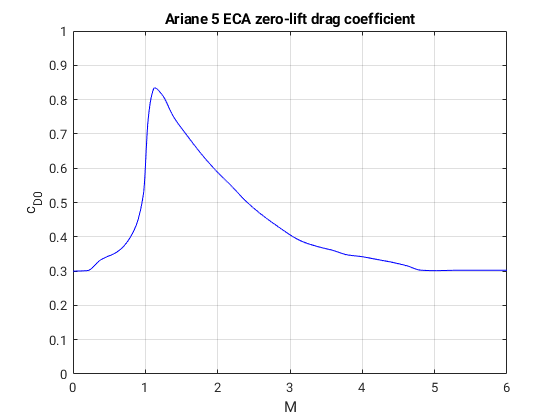
\includegraphics[width=0.735\textwidth]{drag}
 \caption{\emph{Zero-lift drag coefficient}}
 \label{fig:drag}
\end{figure}

\section{Normal force coefficient}
The normal force coefficient is an important parameter, especially for the evaluation of the normal force effect on an aerodynamic model. It must be evaluated since it will be important; moreover, its derivative with respect to the angle of attack is important for the study of a normal aerodynamic force effect and the thrust vector control. From the model described previously, it can be noticed that the cross-section changes along the rocket. To obtain a result in a simple way, consider the coefficient of the two sections separately, and then a weighted average is made with the lengths. The empirical relation adopted is the following: \begin{equation}
 |C_N|=\Biggl[\frac{a}{b}cos^2\phi+\frac{b}{a}sin^2\phi\Biggr]\Biggl[\biggl|sin(2\alpha)cos\biggl(\frac{\alpha}{2}\biggr)\biggr|+1.3\frac{l}{d}sin^2\alpha\Biggr]
\end{equation}
Since the cross section of the rocket changes, a simple approach is to consider the contribution to the coefficient of the upper part with a circular cross section (axisymmetric body), and the lower one with an elliptical cross section (lifting body). Then a weighted averaged will give the final value, weighting on the lengths. The issue is that the empirical relation is valid for a fineness ratio greater than 5, and the respective values for the two parts are both less than 5. So, a single body is considered with the length of the rocket and the elliptical section of the lower part. All the fineness ratios are reported in table \hypertarget{tab:baseline}{\ref{tab:baseline}}. 
\begin{table}[h]
	\centering
	\begin{tabular}{ l l l }
\toprule
%			&$\frac{l}{d}$\\
%\midrule                                                                                                             
Upper part			&$3.7963$\\                                                 
Lower part	        &$3.8069$\\
Overall body		&$6.4083$\\
\bottomrule
\end{tabular} 
\caption{\emph{Fitness ratio $l/d$}}
\label{tab:baseline}
\end{table}\newpage
\noindent It is worth remembering that the aerodynamic coefficients must be referred to the same reference area $(A_{ref})$, that in this case is given by the sum of the \textbf{EPC} area plus the two \textbf{EAP} areas. As a result, the relation becomes: \begin{equation}
 |C_N|=\Biggl[\frac{a}{b}cos^2\phi+\frac{b}{a}sin^2\phi\Biggr]\Biggl[\biggl|sin(2\alpha)cos\biggl(\frac{\alpha}{2}\biggr)\biggr|+1.3\frac{l_B}{2\sqrt{ab}}sin^2\alpha\Biggr]
\end{equation}
The behaviour is shown in figure \hypertarget{fig:normf}{\ref{fig:normf}}. It is worth noting that this relation is not properly correct for this case, also due to the great complexity of the rocket itself; however, it is useful since it gives a good estimation of the normal force coefficient, which will be used, with its derivative with respect to the angle of attack, for the evaluation of the normal aerodynamic force in the plane of the thrust. 
\begin{figure}[h]
 \centering
 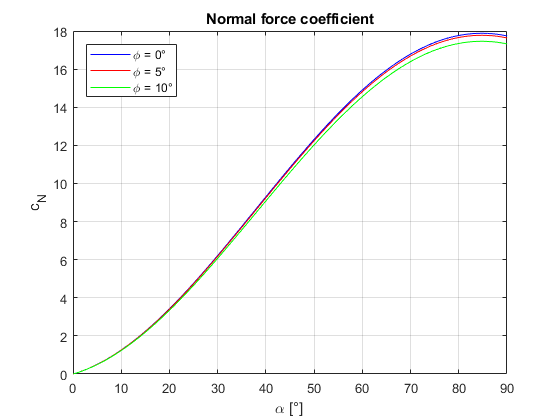
\includegraphics[width=0.75\textwidth]{normf}
 \caption{\emph{Normal force coefficient}}
 \label{fig:normf}
\end{figure}\\
At this point is important to compute the derivative of the normal force coefficient, since it will be useful next: 
\begin{equation}
 C_{N/\alpha}=\frac{\partial}{\partial\alpha}C_N(\alpha,\phi)
\end{equation}
\begin{equation}\begin{split}
 C_{N/\alpha}&=\Biggl[\frac{a}{b}cos^2\phi+\frac{b}{a}sin^2\phi\Biggr]\Biggl[\Biggl|2cos(2\alpha)cos\biggl(\frac{\alpha}{2}\biggr)-\frac{1}{2}sin(2\alpha)sin\biggl(\frac{\alpha}{2}\biggr)\Biggr|+\\
 &+1.3\frac{l_B}{2\sqrt{ab}}2sin\alpha\; cos\alpha\Biggr]
\end{split}\end{equation}
Its behaviour is shown in figure \hypertarget{fig:normfa}{\ref{fig:normfa}}.
\begin{figure}[h]
 \centering
 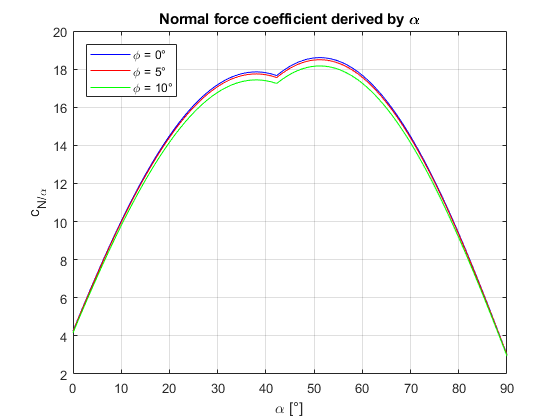
\includegraphics[width=0.75\textwidth]{normfa}
 \caption{\emph{Normal force coefficient derivative}}
 \label{fig:normfa}
\end{figure}
\section{Centre of pressure}
To evaluate the position of the centre of pressure, the slender body theory is adopted and the result is (valid for small angles of attack): 
\begin{equation}
 \frac{x_{CP}}{d}=\underbrace{\frac{2hS}{3dS_b}}_{\text{1}}+\underbrace{\Biggl(1-\frac{S}{S_b}\Biggr)\frac{l_B}{d}}_{\text{2}}-\underbrace{\frac{h_f}{d}\Biggl(\frac{d^2_m}{d^2}-1\Biggr)\frac{S}{S_b}}_{\text{3}}
\end{equation}
In this relation the effects of the nose are considered (1), body (2), and flare (3). To be more precise, but without complicating too much the problem, two values are considered: one related to the main body, and the other related to the boosters. Then a weighted averaged is executed based on the lengths of the two parts. Mathematically: 
\begin{equation}
 \frac{x^{EPC}_{CP}}{d_{EPC}}=\frac{2}{3}\frac{l_N}{d_{EPC}}
\end{equation}
\begin{equation}
 \frac{x_{CP}^{EAP}}{d_{EAP}}=\frac{2}{3}\frac{l_{EAP}A_{EAP}}{d_{EAP}A_f}+\Biggl(1-\frac{A_{EAP}}{A_f}\Biggr)\frac{l_{EAP}}{d_{EAP}}-\frac{h_f}{d_{EAP}}\Biggl(\frac{d^2_m}{d^2_{EAP}}-1\Biggr)\frac{A_{EAP}}{A_f}
\end{equation}
\begin{equation}
 x_{CP}=\frac{x_{CP}^{EPC}(l_B-l_{EAP})+2x_{CP}^{EAP}l_B}{(l_B-l_{EAP})+2l_B}=\SI{19.2756}{m}
\end{equation}
The assumption that the centre of pressure will remain always in that position from the nose of the rocket has been made. 


\chapter{Propulsion}
Since in this report the analysis is focused on the possible troubles given by an imbalance situation between the two external solid rocket boosters, only the first stage of the vehicle is considered. This is composed by the sustainer, called \textbf{EPC} which stands for \textbf{Étage Principal Cryotechnique} that burn parallely with two solid rocket boosters. They are referred to as \textbf{EAPs} from the French Title \textbf{Etage d’Acceleration à Poudre}. This propulsive analysis has two main targets. Firstly, a thrust profile of both \textbf{EAPs} and \textbf{EPC}, as near as possible to the real data, has to be obtained. Secondly, the propellant mass flow rate of the engines has to be computed in order to analyze in the next chapter the excursion of the centre of gravity due to the propellant consumption during the first stage burning time.\\
To reach these goals all the computations are made using the MATLAB\textsuperscript\textregistered software. 
\section{EPC - Étage Principal Cryotechnique}\nomenclature{$I_{sp_{ave}}$}{EAP average specific impulse}
The main core stage of the \textbf{Ariane 5 ECA} provides almost the \SI{8}{\%} of total thrust at liftoff. Is powered by a \textit{Vulcain 2} engine which operates for about \SI{540}{s} burning a mixture of LH2/LOX (Liquid Hydrogen and Liquid Oxygen). Knowing the area expansion ratio, the combustion chamber pressure and the oxidizer to fuel ratio from the literature, using the CEA software from NASA it's possible to calculate the combustion chamber temperature, the molar mass of the combusted gasses and the heat capacity ratio. These data are useful to calculate the specific impulse and the performances of the engine under the hypotesis of frozen conditions.
Velocity and pressure on the nozzle exit section are neeeded to solve the specific impulse relation:
\begin{equation}
 I_{sp}=\frac{V_e}{g_0}+\frac{P_e-P_{amb}}{\rho_eV_e}
\end{equation}
\nomenclature{$I_{sp}$}{Specific Impulse}
\nomenclature{$V_e$}{Velocity of the hot gasses on the nozzle exit section}
\nomenclature{$P_e$}{Pressure of the hot gasses on the nozzle exit section}
\nomenclature{$P_{amb}$}{Ambient pressure}
\nomenclature{$\rho_e$}{Density of the hot gasses on the nozzle exit section}
\nomenclature{$g_0$}{Gravity acceleration}
\noindent In this analysis it is assumed an isentropic model. It's easy to calculate the pressure on the nozzle exit section by using an iterative process starting from the following relation:
\begin{equation}
  \frac{1}{\varepsilon}=\Bigl(\frac{\gamma+1}{2}\Bigr)^{\frac{1}{\gamma-1}}\Bigl(\frac{P_e}{P_{cc}}\Bigr)^{\frac{1}{\gamma}}\sqrt{\Bigl(\frac{\gamma+1}{\gamma-1}\Bigr)\Biggl[1-\Bigl(\frac{P_e}{P_{cc}}\Bigr)^{\frac{\gamma-1}{\gamma}}\Biggr]}              
\end{equation}
\nomenclature{$\varepsilon$}{Area expansion ratio}
\nomenclature{$\gamma$}{Heat capacity ratio}
\nomenclature{$P_{cc}$}{Combustion chamber pressure}
\begin{equation}
  \Bigl(\frac{\gamma+1}{2}\Bigr)^{\frac{1}{\gamma-1}}\Bigl(\frac{P_e}{P_{cc}}\Bigr)^{\frac{1}{\gamma}}\sqrt{\Bigl(\frac{\gamma+1}{\gamma-1}\Bigr)\Biggl[1-\Bigl(\frac{P_e}{P_{cc}}\Bigr)^{\frac{\gamma-1}{\gamma}}\Biggr]}-\frac{1}{\varepsilon}=0              
\end{equation}
Once computed the pressure the next step is to obtain the velocity:
\begin{equation}
 V_e=\sqrt{2\Bigl(\frac{\gamma}{\gamma-1}\Bigr)\frac{R_u}{m_{mol}}T_{cc}\Biggl[1-\Bigl(\frac{P_e}{P_{cc}}\Bigr)^{\frac{\gamma-1}{\gamma}}\Biggr]}
\end{equation}
\nomenclature{$m_{mol}$}{Molar mass of the combusted gasses}
\nomenclature{$T_{cc}$}{Combustion chamber temperature}
Since the propellant total mass and the burning time are known the propellant mass flow rate can be obtained. It's also reasonable to consider it constant beeing the \textit{Vulcain 2} a liquid rocket engine.
\begin{equation}
 \dot{m}_p = \frac{m_p}{t_{burn}}
\end{equation}
\nomenclature{$\dot{m}_p$}{Propellant mass flow rate}
\nomenclature{$m_p$}{Propellant mass}
\nomenclature{$t_{burn}$}{Burning time}
With the last relation the thrust profile vs altitude is computed:
\begin{equation}
 T_{EPC}=\dot{m}_pV_e+(P_e-P_{amb})A_e
\end{equation}
\nomenclature{$A_e$}{Exit section area of the EPC nozzle}
\begin{figure}[h]
 \centering
 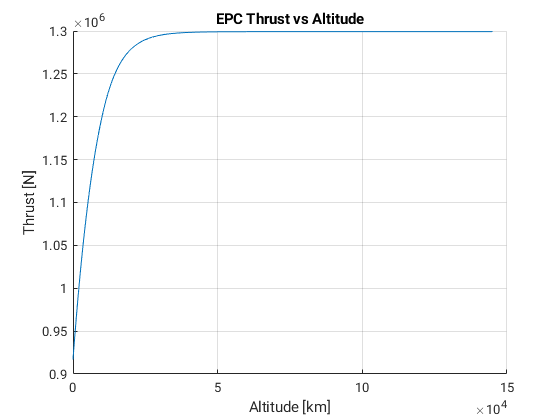
\includegraphics[width=0.75\textwidth]{EPC_T}
 \caption{\emph{EPC Thrust vs Altitude}}
\end{figure}


\section{EAP - Etage d’Acceleration à Poudre}
Parallel to the sustainer two solid rocket boosters burns for about \SI{130}{s}. Powered by HTPB the \textbf{EAPs} provide almost the \SI{92}{\%} of the total thrust at liftoff. Since the thrust in this case depends on the combustion chamber pressure and on the grain geometry it's extremely difficult to compute it analytically. Thanks to the \textit{WebPlotDigitalizer} tool, a web app that allows to extrapolate data from a drawn chart, it's possible to get a set of points representing the thrust profile of the boosters from the original draw as shown in figure \hypertarget{fig:interp}{\ref{fig:interp}}, \cite{bib:8}. Through a linear interpolation the full thrust profile is obtained with a good accuracy.                                     
\begin{comment}
\begin{figure}[h]
 \centering
 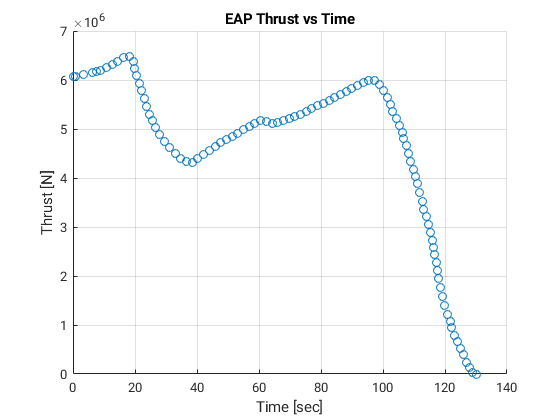
\includegraphics[width=0.85\textwidth]{EAP_T_point}
 \caption{EAP Thrust vs Time - Raw data}
\end{figure}
\begin{figure}[h]
 \centering
 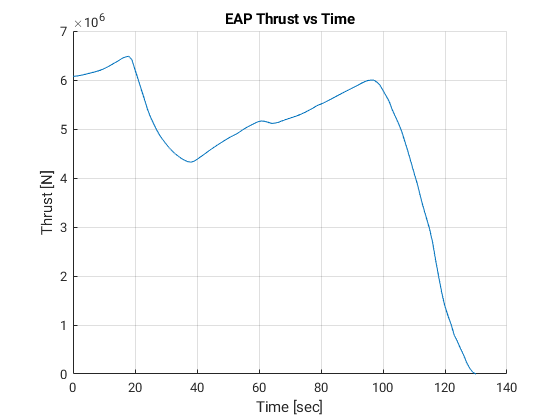
\includegraphics[width=0.85\textwidth]{EAP_T}
 \caption{EAP Thrust vs Time - Linear Interpolation}
\end{figure}\newpage
\end{comment}
\begin{figure}[h]
\centering
\subfloat[][\emph{Raw data}]
{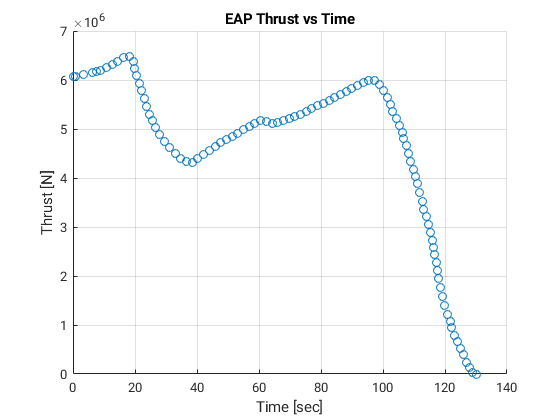
\includegraphics[width=.4805\textwidth]{EAP_T_point}} \quad
\subfloat[][\emph{Interpolation}]
{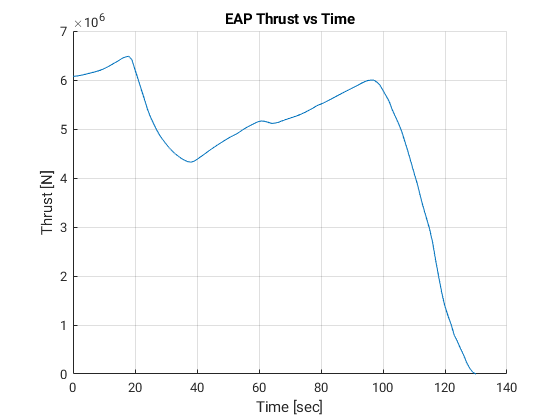
\includegraphics[width=.4805\textwidth]{EAP_T}} \\
\caption{\emph{EAP Thrust profile}}
\label{fig:interp}
\end{figure}
%discorso sullo specific impulse
Assuming an average constant specific impulse, computed from the known data relative to sea level and vacuum conditions, the propellant mass flow rate can be obtained:
\begin{equation}
 I_{sp_{ave}}=\frac{I_{sp_{SL}}+I_{sp_{vac}}}{2}
\end{equation}
\nomenclature{$I_{sp_{ave}}$}{EAP average specific impulse}
\nomenclature{$I_{sp_{SL}}$}{EAP specific impulse at Sea Level}
\nomenclature{$I_{sp_{vac}}$}{EAP specific impulse in vacuum}
\begin{equation}
 \dot{m}_p = \frac{T_{EAP}}{g_0I_{sp_{ave}}}
\end{equation}
\begin{figure}[h]
 \centering
 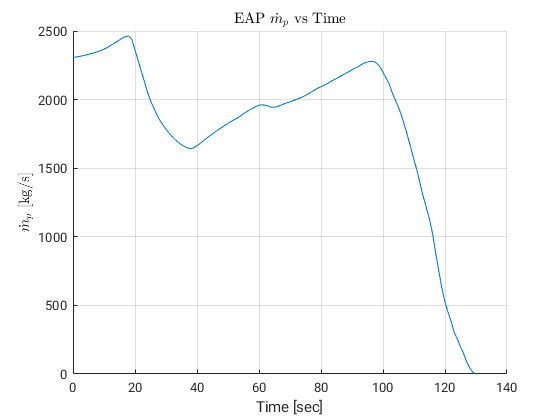
\includegraphics[width=0.7\textwidth]{EAP_mdot}
 \caption{\emph{EAP $\dot{m}_p$ vs Altitude}}
\end{figure}

\chapter{Mass distribution}\label{chap:mass}
Using the data from the baseline, the main parameters have been calculated to evaluate the mass distribution: all the values are reported in table \hypertarget{tab:mdata}{\ref{tab:mdata}}. Through the SolidWorks\textsuperscript\textregistered \\software a CAD model has been realized (\textbf{Ariane 5 ECA} full-of-propellant case, at lift off). By subtracting the mass of propellant used during the different phases of the mission the center of mass has been computed for each case of interest using the software. Two cases were taken under investigation: the one at maximum \textbf{EAP} thrust and the one at maximum dynamic pressure. 

\begin{table}[h]
	\centering
	\begin{tabular}{ l c c c}
\toprule
										&$t=\SI{0}{s}$ 			&$t = \SI{18}{s}$ 		&$t = \SI{71}{s}$	\\
										&[\si{\kilogram}]			&[\si{\kilogram}]			&[\si{\kilogram}]		\\
\midrule                                                                                                             
Main stage hydrogen 					&$24757.143 $			&$24252.8308$			&$21822.943 $		\\
Main stage oxigen 						&$14854.2857$			&$14551.6957$			&$13093.7857$        \\
Booster propellant cylinder shape 		&$214100	   $		&	$175583.760$		&	$85354.600 $        \\
Booster propellant star shape 			&$23150	   $			&$18984.240 $			&$9225.400  $        \\
\bottomrule
\end{tabular} 
\caption{\emph{Propellant mass distribution data}}
\label{tab:mdata}
\end{table}
\noindent At this point it’s requested to know how much propellant mass has to be removed to simulate the shift of the CG. The maximum thrust case corresponds to $time = \SI{18}{s}$. During this phase, using a Matlab\textsuperscript\textregistered code, the consumption of the propellant has been computed (thanks to the mass flow rates). In table \hypertarget{tab:maxEAP}{\ref{tab:maxEAP}} are reported the results. 
\begin{table}[h]
	\centering
	\begin{tabular}{ l c c c}
\toprule
										&$LH_2$ 			&$LOX$ 				&$Booster$	\\
										&[\si{\kilogram}]			&[\si{\kilogram}]			&[\si{\kilogram}]		\\
\midrule                                                                                                             
Mass burned								&$504.3122$			&$3025.9$			&$42682$			\\
\bottomrule
\end{tabular} 
\caption{\emph{Maximum EAP thrust condition at \SI{18}{s}}}        
\label{tab:maxEAP}                       
\end{table}                             
                      
\noindent Removing the corresponding part of propellant, taking in account its burning behavior, from the full-of-propellant case, the center of gravity results to be at \SI{16.2341}{m} (from the base of the launcher). It can be noticed that the top part of the \textbf{EAP} has a star-shaped component, that guarantees the higher thrust profile. The maximum dynamic pressure case corresponds to $time = \SI{71}{s}$. In an analogous way to the maximum thrust case, the mass of propellant burned has been found. In table \hypertarget{tab:maxP}{\ref{tab:maxP}} are reported the results.  

\begin{table}[h]
	\centering
	\begin{tabular}{ l c c c}
\toprule
										&$LH_2$ 			&$LOX$ 				&$Booster$	\\
										&[\si{\kilogram}]			&[\si{\kilogram}]			&[\si{\kilogram}]		\\
\midrule                                                                                                             
Mass burned								&$2934.2$			&$17605$			&$142670$			\\
\bottomrule
\end{tabular} 
\caption{\emph{Maximum dynamic pressure condition at \SI{71}{s}}}        
\label{tab:maxP}                       
\end{table} 
\noindent Removing the corresponding part of propellant from the full-of-propellant case, the center of gravity results to be at \SI{17.3815}{m}. In particular, it can be noticed that the top part of the \textbf{EAP} is no more star-shaped. The resulting mass distributions inside the rocket for the two cases are shown in figure \hypertarget{fig:subfigA5}{\ref{fig:subfigA5}}. 
\begin{figure}[h]
\centering
\subfloat[][\emph{Mass distribution at \SI{18}{s}}]
{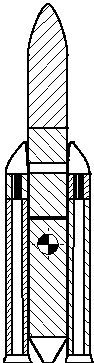
\includegraphics[width=.2\textwidth]{A5m1}} \quad
\subfloat[][\emph{Mass distribution at \SI{71}{s}}]
{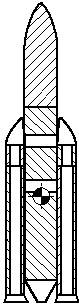
\includegraphics[width=.2\textwidth]{A5m2}} \\
\caption{\emph{Ariane 5-ECA mass distribution}}
\label{fig:subfigA5}
\end{figure}

\chapter{Thrust vector control}
At this point it’s important to analyse the effect of the imbalance on the rocket when flying at a certain attitude and altitude. The effect of a normal aerodynamic force \textit{N} in two critical cases is analyzed: maximum \textbf{EAP} thrust and maximum dynamic pressure. In addition, for each case it’s considered the shift of the \textit{CG} of the rocket after the burning of the propellant for each of the two conditions: the evaluation of \textit{CG} was obtained in chapter \hypertarget{chap:mass}{\ref{chap:mass}}. The results on the deflection angles of all the three nozzles (1 \textbf{EPC}, 2 \textbf{EAP}) are shown. First, it will be analysed the imbalance modelling. The maximum deflection angles for the nozzles are reported in table \hypertarget{tab:maxang}{\ref{tab:maxang}}. 
\begin{table}[h]
	\centering
	\begin{tabular}{ l c }
\toprule
										&Maximum deflection angle 				\\
										&[\si{\degree}]			\\
\midrule                                                                                                             
$\delta_{EPC}^{max}$						&$7$			\\
$\delta_{EAP}^{max}$						&$7.3$			\\
\bottomrule
\end{tabular} 
\caption{\emph{EAP and EPC engines maximum deflection angles}}        
\label{tab:maxang}                       
\end{table}
\section{Imbalance}
The imbalance is defined as the difference between the thrust given by the two external boosters:
\begin{equation}
	\Delta T = T_1-T_2
\end{equation}
To model it simply, it is considered a maximum value of imbalance equal to the 5\% of the thrust of the single SRM. First random variations of the thrust for the two SRMs are created, but different, with a maximum value of $\pm\SI{2.5}{\%}$. Then, they are subtracted to give a random thrust imbalance. 1000 samples will be considered, with zero mean and $1\sigma$ of standard deviation, using the function \textit{rand} of Matlab\textsuperscript\textregistered: in this way the level of thrust change will be equally distributed. Mathematically it means:
\begin{equation}
	\Delta T_1=0.025+0.05rand(1000,1)
\end{equation}
\begin{equation}
	\Delta T_2=0.025+0.05rand(1000,1)
\end{equation}
\begin{equation}
    \Delta T = \Delta T_1-\Delta T_2
\end{equation}
In this way the imbalance can be given by a random effect of increasing or decreasing thrust of both the SRMs. It is important to underline that the two random parameters are considered uncorrelated. The thrust imbalance has been redefined to be consistent with the figures shown in the next chapter, so as percentage with respect to the nominal value $T_{EAP}$. 
\section{Maximum EAP thrust}
The first case analysed is the condition of maximum \textbf{EAP} thrust. It will be considered the imbalance together with the stability against the action of the normal aerodynamic force: the scheme for this case is shown in figure \hypertarget{fig:A5sch}{\ref{fig:A5sch}}, where positive rotations are counter clockwise (also for the deflection angles). The normal aerodynamic force is considered to give more generality to the analysis. It is worth noting that the variation of $\alpha$ simulates an increasing effect of the normal force, to be analysed. The approach followed is the subsequent. First it is rotated the nozzle of the \textbf{EPC} to counteract the aerodynamic force. Then it is rotated the proper SRM nozzle to counteract the imbalance. Since there is a limit on the deflection angle of the \textbf{EPC}, when it is exceeded, it is set to the maximum value possible and then the two SRM nozzles are rotated together, analysing if they are able to counteract the normal force. A \textit{two degrees of freedom model} has been selected for this design. 
\begin{figure}[h]
 \centering
 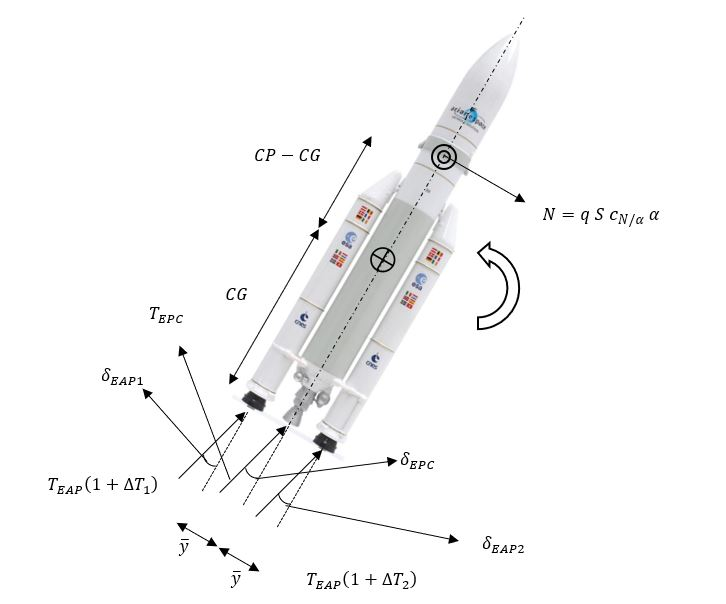
\includegraphics[width=0.85\textwidth]{TVC}
 \caption{\emph{Ariane 5 ECA TVC scheme}}
 \label{fig:A5sch}
\end{figure}\newpage
\noindent The conditions and parameters are reported in table \hypertarget{tab:maxEAPpar}{\ref{tab:maxEAPpar}}, coming from aerodynamics, propulsion, and mass distribution.
\begin{table}[h]
	\centering
	\begin{tabular}{ l r }
\toprule
Parameter					&Value 				\\
%							&\si{\degree}			\\
\midrule                                                                                                             
$Time\; after\; launch$			&\SI{18}{s}			\\
$Altitude$					&\SI{394.7}{m}      \\
$CG\;\; position\; from\; the\; base$	&\SI{16.2341}{m}    \\
$CP-CG $				&\SI{14.9903}{m}    \\
$\bar{y}$ 					&\SI{4.225}{m}      \\
$T_{EAP}$						&\SI{6.485}{MN}     \\
$T_{EPC}$						&\SI{0.9345}{MN}    \\
$q$							&\SI{4.686}{kPa}    \\
\bottomrule
\end{tabular} 
\caption{\emph{Parameters for maximum EAP thrust}}        
\label{tab:maxEAPpar}                       
\end{table}\\
It is considered the equilibrium around the \textit{CG} of the rocket. To counteract the aerodynamic force, the subsequent reasoning has been followed: 
\begin{enumerate}
 \item Rotate the \textbf{EPC} nozzle without rotating the SRM nozzles, using the following relation:\\
 \begin{equation}
  sin(\delta_{EPC})=\frac{qA_{ref}}{T_{EPC}CG}C_{N/\alpha}(CP-CG)\alpha
 \end{equation}
 where the angle of attack is positive, and $C_{N/\alpha}$ is evaluated in $(\alpha,0)$.\\
 \item If the imbalance is positive $(\Delta T_1>\Delta T_2)$, it’s rotating the left nozzle clockwise to compensate it, obtaining:\\
 \begin{equation}\begin{split}
  &-T_{EAP}(1+\Delta T_1)cos(\delta_{EAP1})\bar{y}+T_{EAP}(1+\Delta T_1)sin(\delta_{EAP1})CG+\\
  &+T_{EAP}(1+\Delta T_2)\bar{y}=0
 \end{split}\end{equation}
 while if the imbalance is negative $(\Delta T_1<\Delta T_2)$ rotates the other counter clockwise, obtaining: \\
 \begin{equation}\begin{split}
  &-T_{EAP}(1+\Delta T_1)\bar{y}+T_{EAP}(1+\Delta T_2)cos(\delta_{EAP2})\bar{y}+\\
  &-T_{EAP}(1+\Delta T_1)sin(\delta_{EAP2})CG=0
 \end{split}\end{equation}
 The resulting deflection angle is obtained, using the function \textit{fsolve} of Matlab\textsuperscript\textregistered.\\
 \item If the limiting value of the \textbf{EPC} nozzle is overcome, the other two nozzles are rotated simultaneously to compensate the remaining moment. This is done solving the following equation of balance (again using \textit{fsolve}): 
 \begin{equation}\begin{split}
  &T_{EPC}sin(\delta_{EPC}^{max})CG+T_{EAP}(1+\Delta T_1)sin(\delta_{EAP1}+\delta)CG+ \\
  -&T_{EAP}(1+\Delta T_1)cos(\delta_{EAP1}+\delta)\bar{y}+\\
  +&T_{EAP}(1+\Delta T_2)sin(\delta_{EAP2}+\delta)CG+ \\
  +&T_{EAP}(1+\Delta T_2)cos(\delta_{EAP2}+\delta)\bar{y}-qA_{ref}C_{N/\alpha}(CP-CG)\alpha=0
 \end{split}
 \end{equation}
 where $\delta$ is the angle of which rotate the two SRM nozzles. Then this angle is added properly to the previous value resulting from the imbalance.\\
 \item Then it is evaluated also the ideal thrust without imbalance, along the axis of the rocket: 
 \begin{equation}
  T_{EPC}\;sin(\delta_{EPC})CG+2T_{EAP}sin(\hat{\delta})-qA_{ref}C_{N/\alpha}(CP-CG)\alpha=0
 \end{equation}
 and from $\hat{\delta}$, which is the angle of which rotate the two SRMs without imbalance: 
 \begin{equation}
  T_{ideal}=T_{EPC}\;cos(\delta_{EPC})+2T_{EAP}\;cos(\hat{\delta})
 \end{equation}
 \item Finally, the resulting real thrust is obtained as:
 \begin{equation}\begin{split}
  &T=T_{EPC}\;cos(\delta_{EPC})+T_{EAP}(1+\Delta T_1)cos(\delta_{EAP1})+\\
  +&T_{EAP}(1+\Delta T_2)cos(\delta_{EAP2})
 \end{split}\end{equation}
 \end{enumerate} 
 At this point, for the simulation five values for the angle of attack are considered:\\ $\SI{0}{\degree}, \SI{3}{\degree}, \SI{5}{\degree}, \SI{7}{\degree}, \SI{10}{\degree}$. 


\section{Maximum dynamic pressure}
 The second condition is that of maximum dynamic pressure. The conditions and parameters are reported in table \hypertarget{tab:maxq}{\ref{tab:maxq}}. It will be followed the same procedure seen before.
\begin{table}[h]
	\centering
	\begin{tabular}{ l c }
\toprule
Parameter					&Value 				\\
%							&\si{\degree}			\\
\midrule                                                                                                             
$Time\; after\; launch$			&\SI{71}{s}			\\
$Altitude$					&\SI{14570}{m}      \\
$CG\; position\; from\; the\; base$	&\SI{17.3815}{m}    \\
$CP-CG $				&\SI{13.8428}{m}    \\
$\bar{y}$ 					&\SI{4.225}{m}      \\
$T_{EAP}$						&\SI{5.242}{MN}     \\
$T_{EPC}$						&\SI{1.251}{MN}    \\
$q$							&\SI{34}{kPa}    \\
\bottomrule
\end{tabular} 
\caption{\emph{Parameters for maximum dynamic pressure}}        
\label{tab:maxq}                       
\end{table}

\chapter{Results and Conclusions}
By the previous analysis, the needed TVC deflection angles to compensate a random thrust imbalance are obtained as main result. These results focus on two fundamental flight phases performed by the complete configuration of \textbf{Ariane 5 ECA} (main body + boosters):
\begin{enumerate}
 \item Max boosters thrust phase (time of flight $t = \SI{18}{s}$)
 \item Max dynamic pressure (time of flight $t=\SI{71}{s}$)\\
\end{enumerate}
 First consider the case of maximum \textbf{EAP} thrust condition. In this case the dynamic pressure has a low value and the associated normal aerodynamic force will be not so large. In figure \hypertarget{fig:emaxt}{\ref{fig:emaxt}} it is shown the deflection angle of the \textbf{EPC} motor used to counteract the normal force. As it can be seen, up to \SI{5}{\degree} is able alone to counteract it. Then, it’s necessary to use also the two boosters. In figures \hypertarget{fig:emaxtl}{\ref{fig:emaxtl}} and \hypertarget{fig:emaxtr}{\ref{fig:emaxtr}} the deflection angles are shown for the left and the right \textbf{EAP} nozzles respectively. In this case the results show that there are no problems in counteracting the normal force, also at \SI{10}{\degree}, since the limiting value is never reached. For a positive imbalance, the deflection angle of the left nozzle must be rotated more (counter clockwise), and the resulting value keeps increasing. In the opposite case, the value keeps decreasing since the right nozzle rotates clockwise. The value at $\Delta T = 0$ is the one at which the two \textbf{EAPs} nozzles should be rotated to counteract \textit{N} together with the \textbf{EPC} one, without imbalance. \\ 
 In the second case, the level of the \textbf{EAP} thrust is reduced (not too much), but the dynamic pressure is very high: the situation is definitely different. At zero angle of attack the imbalance is counteracted by a proper deflection of boosters’ nozzles while at all the other considered angles the \textbf{EPC’s} nozzle deflective capability is saturated. From figure \hypertarget{fig:emaxq}{\ref{fig:emaxq}} it is evident that the \textbf{EPC} nozzle isn’t able alone to counteract the normal force; so, the EAP nozzle must be rotated. From figures \hypertarget{fig:emaxql}{\ref{fig:emaxql}} and \hypertarget{fig:emaxqr}{\ref{fig:emaxqr}} it can be noticed that up to \SI{7}{\degree} is again possible to counteract the normal force, even if almost close to the limiting deflection angles. Then, at \SI{10}{\degree} the limiting values are exceeded: in this situation it’s very likely that the mission would result in a complete loss of the launcher. However, \SI{10}{\degree} is typically a high value for a rocket, and it has been introduced as an upper limit for this study.  
 Same considerations, as done before, for the different situations it's easy to deduce that the most demanding condition in terms of attitude control by TVC is the maximum dynamic pressure situation. This is true for the whole flight phase and not only for the phases analysed previously.
 \newpage \noindent The previous study may be improved by adding complexities to the used models already described in order to pass from a conceptual analysis to a design phase one. In particular these changes in modelling may be applied to obtain a more complete analysis:
 \begin{itemize}
  \item \textbf{More complex aerodynamic model:} the aerodynamic model used to evaluate fluid dynamics effects on the launcher is a very general one and it is based on assumptions that are brought to their limits by the \textbf{Ariane 5 ECA} shape and configuration. An ad hoc aerodynamic model based on the launcher shapes would be far more effective in foreseeing the effective aerodynamic loads on the launcher. Also, the analysis of the generated aerodynamic moments due to the launcher shape should be added to perform a more precise analysis.
  \item \textbf{Elastic body model of the launcher and mechanical peculiar behaviours:} the launcher has been considered throughout the previous analysis as a perfect rigid body in order to avoid the study of its structural dynamics. Surely mechanical couplings may affect the attitude of the launcher during flight. In addition, the rotation of the nozzles has been considered as perfectly matching the needed rotation to counteract the imbalance while uncertainties should affect it. The TVC system introduces some changes in the structural load distribution on the launcher that should be considered to perform a more complete study. 
  \item \textbf{Main engine performances uncertainties}: the main engine performances are considered as exactly matching the nominal ones. In reality some uncertainties about them should be considered as well as the uncertainties about the boosters’ performances have been considered in this work. Main engine performances uncertainties would not generate an imbalance moment, but they may affect the overall performances of the launcher.
 \end{itemize}
 For a next iteration of the conceptual design phase, some changes should be made. The reason is that, even if the requirements are satisfied, at \SI{7}{\degree} the deflection angles of the SRMs are close to the limiting values; so, a more precise aerodynamic model and the introduction of the pitch moment coefficient (\textit{three degrees of freedom pitching}) could reveal if the system is again able to counteract the normal force. 
\\ \\ \\ \\ \\ \\ \\ \\ \\ \\ \\ \\
 \begin{figure}[h]
 \centering
 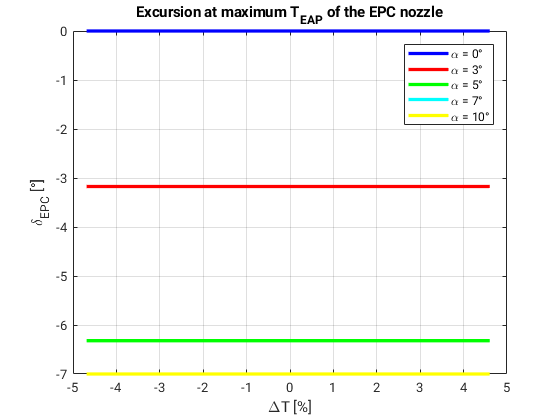
\includegraphics[width=0.75\textwidth]{emaxT}
 \caption{\emph{Excursion at maximum EAP thrust of the EPC nozzle}}
 \label{fig:emaxt}
\end{figure}
\begin{figure}[h]
 \centering
 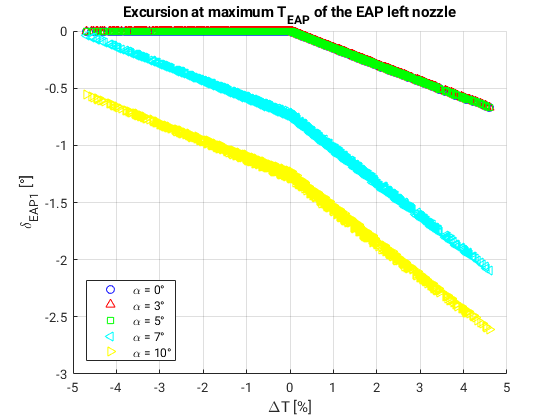
\includegraphics[width=0.75\textwidth]{emaxTl}
 \caption{\emph{Excursion at maximum EAP thrust of the EAP left nozzle}}
 \label{fig:emaxtl}
\end{figure}
\begin{figure}[h]
 \centering
 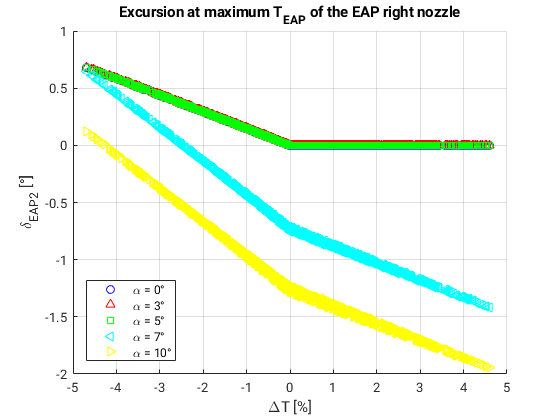
\includegraphics[width=0.75\textwidth]{emaxTr}
 \caption{\emph{Excursion at maximum EAP thrust of the EAP right nozzle}}
 \label{fig:emaxtr}
\end{figure}
 %IMAGESS
 \begin{figure}[h]
 \centering
 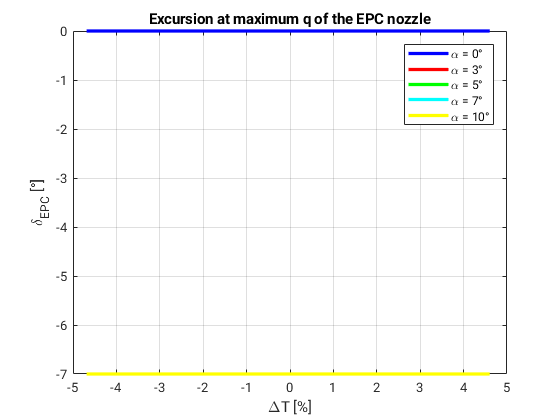
\includegraphics[width=0.75\textwidth]{emaxq}
 \caption{\emph{Excursion at maximum q of the EPC nozzle}}
 \label{fig:emaxq}
\end{figure}
\begin{figure}[h]
 \centering
 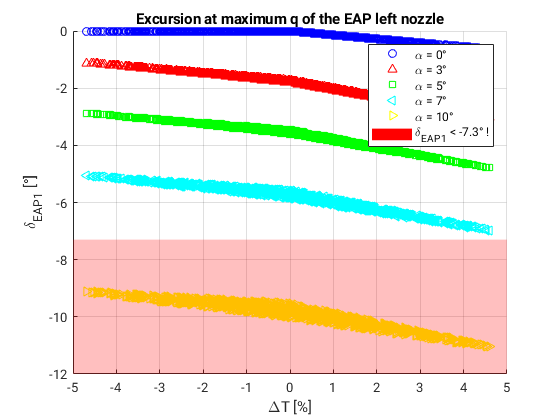
\includegraphics[width=0.75\textwidth]{emaxql}
 \caption{\emph{Excursion at maximum q of the EAP left nozzle}}
 \label{fig:emaxql}
\end{figure}
\begin{figure}[h]
 \centering
 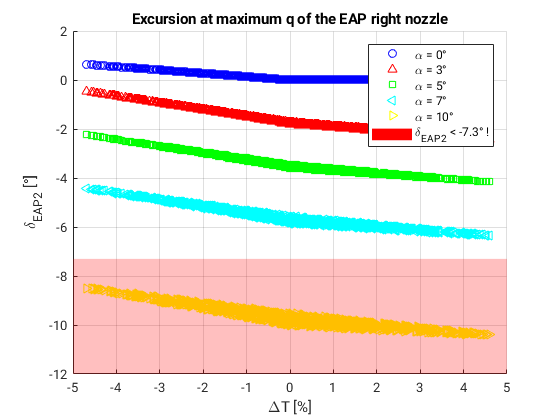
\includegraphics[width=0.75\textwidth]{emaxqr}
 \caption{\emph{Excursion at maximum q of the EAP right nozzle}}
 \label{fig:emaxqr}
\end{figure}

\clearpage
\addcontentsline{toc}{chapter}{\bfseries{\bibname}}
\begin{thebibliography}{9}
	\bibitem{bib:1}{W.A. Foster, R.H. Sforzini, B.W. Schackelford, \emph{Thrust Imbalance of the Space Shuttle Solid Rocket Motors}, AIAA, AIAA Paper 2014-12532}
	\bibitem{bib:2}{W.A. Foster, R.H. Sforzini, P.H. Shu, \emph{Thrust Imbalance of Solid Rocket Motors Pairs on Space Shuttle Flights}, AIAA, AIAA Paper 1986-1375}
	\bibitem{bib:3}{W.A. Foster, W. Crowder, T.E. Steadman, \emph{A Monte Carlo Analysis of the Thrust Imbalance for the Space Launch System Booster during Both the Ignition Transient and Steady State Operation}, AIAA, AIAA Paper 2014-12532}
	\bibitem{bib:4}{\url{www.spaceflight101.com/ariane-5-va226/ariane-5-va226-launch-profile}}
	\bibitem{bib:5}{Ariane 5 User’s Manual, \url{www.arianespace.com/vehicle/ariane-5/}}
	\bibitem{bib:6}{Safran (Snecma), Fiche vulcain2 vulcain ang 2011.pdf}
	\bibitem{bib:7}{F. Castellini, A. Riccardi, M. Lavagna, C. Büskens, \emph{Global and Local Multidisciplinary Design Optimization of Expendable Launch Vehicles}, report 11-09, $December\;2011$}
	\bibitem{bib:8}{A5prop.pdf}
\end{thebibliography}


\end{document}   